\documentclass[conference]{IEEEtran}
\IEEEoverridecommandlockouts
% ---------------------------------------------------------------
% Packages
% ---------------------------------------------------------------
\usepackage{cite}
\usepackage{amsmath,amssymb,amsfonts}
\usepackage{algorithmic}
\usepackage{graphicx}
\usepackage{multirow}
\usepackage{textcomp}
\usepackage{xcolor}
\usepackage{tikz}
\usetikzlibrary{arrows.meta, positioning, calc}
\usepackage{url}
\usepackage[hidelinks]{hyperref}

\def\BibTeX{{\rm B\kern-.05em{\sc i\kern-.025em b}\kern-.08em
    T\kern-.1667em\lower.7ex\hbox{E}\kern-.125emX}}

\begin{document}

% =================================================================
% Title, authors, and affiliations
% =================================================================
\title{A Multilingual Comparative Evaluation of Zero-Shot Voice Cloning Architectures for English and Hindi Speech Synthesis}

\author{
\IEEEauthorblockN{Samaksh Gupta}
\IEEEauthorblockA{\textit{Computer Science and Engineering} \\
\textit{Manipal University Jaipur} \\
Jaipur, India \\
samakshgupta04@gmail.com}
\and
\IEEEauthorblockN{Dhairya Yadav}
\IEEEauthorblockA{\textit{Computer Science and Engineering in DS} \\
\textit{Bhilai Institute of Technology} \\
Bhilai, India \\
dhairyayadavg@gmail.com}
\and
\IEEEauthorblockN{TODO}
\IEEEauthorblockA{\textit{Add more authors} \\
\textit{-} \\
- \\
-}
}
\maketitle

% =================================================================
% Abstract
% =================================================================
\begin{abstract}
Zero-shot voice cloning has improved rapidly, but the way these systems are
evaluated has not kept up. Published benchmarks usually cover a single
high-resource language, report one quality metric, and rarely compare
architecturally different systems under the same conditions. Hindi in
particular tends to appear only as one entry in a multilingual training
mixture rather than as the subject of a dedicated study. We compare three
recent systems that differ in how speaker identity enters the model:
Orpheus-3B, which prepends the reference audio as a token prefix to an LLM
backbone; VoxCPM2, which cross-attends to a fixed speaker prototype; and
VibeVoice, a diffusion decoder guided by a contrastive speaker encoder. All
three receive the same 25.5-second reference recording and the same twelve
English and Hindi utterances, and all outputs are scored by the same three
pipelines: speaker-embedding cosine similarity, Whisper-based word and
character error rates, and UTMOS naturalness prediction. None of the systems
is best on every metric. VoxCPM2 preserves speaker identity and pitch register
most accurately and produces the most intelligible speech in both languages.
VibeVoice scores highest on naturalness and degrades the least from English to
Hindi, but is unreliable on exact content such as digits and alphanumeric
codes. Orpheus-3B is weakest on identity and pitch. Within each system, the
English and Hindi speaker-similarity means differ by at most 0.005 even though
intelligibility drops sharply, which suggests that a large part of the
measured Hindi error comes from the ASR and romanization steps of the scoring
pipeline rather than from the synthesis itself. On this protocol, persistent
cross-attention to a speaker prototype was a more reliable identity mechanism
than an autoregressive prefix.
\end{abstract}

\begin{IEEEkeywords}
zero-shot voice cloning, text-to-speech, speaker verification, multilingual speech synthesis, Hindi TTS, neural codec language models
\end{IEEEkeywords}

% =================================================================
% Section I: Introduction
% =================================================================
\section{Introduction}
\label{sec:introduction}

Text-to-speech synthesis has progressed from rule-based concatenative methods
to neural models whose output is often difficult to distinguish from recorded
speech. Zero-shot voice cloning pushes this further: given a short reference
recording, typically 20 to 30 seconds of natural speech, the model must
reproduce that speaker's voice on arbitrary new text without any
speaker-specific fine-tuning. This requires more than accurate signal
reconstruction. To carry a voice onto sentences the reference speaker never
actually said, the model has to separate speaker-characteristic properties
(timbre, prosodic habits, vocal tract resonance) from the linguistic content.
Orpheus-3B \cite{orpheus2024}, VoxCPM2 \cite{voxcpm2024}, and VibeVoice
\cite{vibevoice2024} approach that separation in structurally different ways,
and the aim of this paper is to measure how those design choices behave under
one controlled comparison.

Neural codec language models \cite{wang2023neural, borsos2023audiolm},
flow-matching decoders \cite{le2024voicebox}, and diffusion-based vocoders
have produced zero-shot systems whose mean opinion scores approach
ground-truth recordings, at least in controlled English evaluations.
Evaluation practice has been less consistent. Most published benchmarks use
clean studio-quality reference audio, target one high-resource language, and
report MOS under conditions that may not reflect deployment. The situation is
worse in multilingual settings. Hindi is spoken by more than 600 million
people, but its phonological properties, including retroflex consonants,
contrastive vowel nasalization, and an ambiguous Devanagari-to-phoneme
mapping, make both acoustic modeling and ASR-based intelligibility scoring
harder than the English case that most benchmarks are built around. A model
with a low English word error rate (WER) can still fail badly on Hindi if its
architecture was never trained on phonologically diverse corpora.

Speaker identity preservation adds a second difficulty. A 20--30 second clip
carries only so much speaker-specific information, and the model has to
extract a stable representation from that limited evidence and hold onto it
across target sentences of varying length and phonetic content. On the
measurement side, cosine similarity between embeddings from an independent
speaker encoder (a GE2E d-vector network, for instance) gives a reproducible
proxy for perceptual identity, although it does not capture every dimension of
how listeners recognize a voice. Naturalness is just as hard to measure at
scale. Neural MOS predictors such as UTMOS \cite{saeki2022utmos} avoid the
cost of human listening panels, but how well they transfer across languages
remains an open question.

In this work we evaluate three contemporary zero-shot voice cloning systems:
\textbf{Orpheus-3B} \cite{orpheus2024}, a large language model-based TTS
system adapted for zero-shot speaker conditioning; \textbf{VoxCPM2}
\cite{voxcpm2024}, a codec-based generative model trained on diverse
multilingual speech; and \textbf{VibeVoice} \cite{vibevoice2024}, a
diffusion-based synthesis pipeline with a contrastive speaker encoder. Each
system receives an identical 20-to-30 second reference clip and the same
target texts. Outputs are scored on three complementary axes: speaker
similarity (cosine distance in speaker embedding space), intelligibility
(Word Error Rate for English and Character Error Rate for Hindi, both
transcribed with Whisper \cite{radford2023whisper}), and acoustic naturalness
(UTMOS). We use CER rather than WER for Hindi deliberately: Whisper's Hindi
output shows transliteration inconsistencies at word boundaries, and
character-level comparison separates phoneme fidelity from tokenization
artifacts.

The comparison matters beyond benchmarking because each architecture makes
different assumptions about the speaker conditioning mechanism, the decoder,
and the training regime. Orpheus-3B conditions generation autoregressively
through a speaker-prefixed token sequence; VoxCPM2 uses cross-attention to a
speaker prototype inside a codec language model; VibeVoice guides a diffusion
process with a contrastive speaker embedding. Knowing which of these holds
identity more stably from a short reference, and whether that stability
carries across scripts, is useful both for choosing a model to deploy and for
deciding which architectural directions are worth pursuing in multilingual
TTS research.

The rest of the paper is organized as follows. Section~\ref{sec:related}
reviews related work on neural TTS, zero-shot speaker adaptation, and
multilingual synthesis. Section~\ref{sec:methodology} describes the
experimental setup, including the corpus, preprocessing, and metric
implementations. Section~\ref{sec:results} presents the quantitative results,
Section~\ref{sec:discussion} analyzes the observed trade-offs and their
architectural correlates, and Section~\ref{sec:conclusion} summarizes the
findings and outlines future work.

% =================================================================
% Section II: Related Work
% =================================================================
\section{Related Work}
\label{sec:related}

\subsection{The Evolution of Zero-Shot Voice Cloning}
\label{sec:related-evolution}

Early neural TTS systems such as Tacotron \cite{wang2017tacotron} and
Tacotron-2 \cite{shen2018natural} treated speaker identity as fixed at
training time. They raised naturalness considerably, but they could only
produce the voices they had been trained on, and supporting a new speaker
meant retraining. Cloning an unseen voice requires the model to separate
speaker identity from linguistic content in some explicit or implicit way.

Jia et al.~\cite{jia2018transfer} showed that embeddings from a pretrained
speaker-verification network could condition a synthesizer on a new voice
from only a few seconds of audio. Arik et al.~\cite{arik2018neural} examined
the trade-off inherent in this approach: an external speaker encoder allows
adaptation without retraining, while fine-tuning the synthesizer itself gives
better quality for that one speaker at much higher cost.

Later systems such as VITS \cite{kim2021vits} and FastSpeech-2
\cite{ren2020fastspeech2} improved quality and inference speed but kept the
same basic separation. YourTTS \cite{casanova2022yourtts} extended it by
training across many speakers and languages simultaneously, which improved
zero-shot behavior, though quality remained limited mostly by what the
speaker encoder could represent rather than by the synthesizer itself.

A larger shift came from reframing TTS as language modeling over discrete
audio tokens. VALL-E \cite{wang2023neural} showed that an autoregressive
transformer over neural codec tokens can clone a voice through in-context
prompting alone: the reference clip is placed before the target text, and the
continuation inherits the speaker without any explicit embedding bottleneck.
This built on the hierarchical token modeling that AudioLM
\cite{borsos2023audiolm} had introduced for general audio.

The systems that followed mostly kept the token representation and changed
the decoding procedure. Voicebox \cite{le2024voicebox} replaced autoregression
with flow matching over masked spans, allowing faster non-causal infilling.
NaturalSpeech~3 \cite{ju2024naturalspeech3} factorized content, prosody, and
timbre into separate discrete subspaces. TorToise \cite{betker2023better}
showed that simply scaling a fairly standard diffusion-decoder pipeline
closes much of the remaining naturalness gap without architectural novelty.

The three systems evaluated here sit at different points on this trajectory.
Orpheus-3B \cite{orpheus2024} follows the VALL-E approach but builds directly
on a pretrained LLM backbone, with the reference speaker supplied as a token
prefix, so cloning depends entirely on the language model's in-context
learning. VoxCPM2 \cite{voxcpm2024} keeps the codec-language-model design but
replaces the prefix with cross-attention to a fixed speaker prototype, an
intermediate point between pure prompting and an explicit embedding.
VibeVoice \cite{vibevoice2024} departs from autoregressive codec modeling
altogether and uses a diffusion decoder conditioned on a contrastively
trained speaker encoder, which places it closer to representation-learning
systems such as StyleTTS~2 \cite{li2023styletts2}.

That three recent production-grade models disagree this much about how
identity should be injected suggests the field has not settled on a
conditioning mechanism. This is the main reason a side-by-side evaluation
seemed worthwhile to us: results reported separately, on different data and
different metrics, do not answer the question.

\subsection{Cross-Lingual and Multilingual Generalization}
\label{sec:related-multilingual}

Most of the zero-shot cloning literature is anchored to datasets and
evaluation protocols built around a handful of high-resource, mostly
Latin-script languages. YourTTS \cite{casanova2022yourtts} was among the
first to report cross-lingual cloning and found that transferring a speaker
into a typologically distant language costs more naturalness than transfer
within a related family. XTTS \cite{casanova2024xtts} scaled multilingual
pretraining substantially further, but its language pool still concentrates
on Indo-European and East Asian languages, with lower-resource languages
evaluated as secondary conditions rather than as the subject of the study.
VALL-E~X \cite{zhang2023speak} addressed the cross-lingual case directly by
training a shared codec language model on English and Mandarin, and reported
a measurable loss of speaker similarity when an embedding learned on one
phonetic inventory has to generalize to another.

Hindi is further from English than the pairs typically studied. It has
retroflex stops that English lacks, contrastive vowel nasalization, and
schwa-deletion rules that make a Devanagari grapheme sequence an unreliable
guide to the phonemes actually produced. Extending the VALL-E~X observation
to Hindi is therefore not just a matter of adding training data in a new
language; it tests whether the conditioning mechanism itself is
language-invariant.

Indic-language speech technology has largely developed as a separate
resource-building effort rather than in dialogue with the cloning literature
above. AI4Bharat's work at national-language scale, spanning ASR
\cite{javed2022towards}, standardized recognition benchmarking
\cite{bhogale2023vistaar}, and large multi-task speech corpora
\cite{javed2024indicvoices}, is oriented toward recognition rather than
generation, and earlier end-to-end Indian-language TTS
\cite{prakash2019building} depended on hours of curated single-speaker
recordings, the opposite of the 20--30 second zero-shot setting adopted here.
Zero-shot cloning results specific to Hindi remain sparse. Models often list
Hindi among many training languages, but they rarely report Hindi speaker
similarity, intelligibility, and naturalness with the same rigor as their
English numbers, so it is hard to tell whether claimed multilingual
competence reflects genuine phonological robustness or simply the composition
of the pretraining corpus.

\subsection{The Transition to Automated Evaluation Pipelines}
\label{sec:related-evaluation}

For most of neural TTS history, the mean opinion score (MOS) listening test
was the accepted arbiter of quality, but crowdsourced MOS collection has
known reliability problems. Ribeiro et al.~\cite{ribeiro2011crowdmos}
documented substantial rater variance in crowdsourced studies, and Cooper et
al.~\cite{cooper2022generalization} showed that a MOS predictor trained on
one listening-test population does not reliably transfer to different
conditions, which undermines comparisons against scores quoted from prior
work. Running a separate listening panel for every system is also expensive;
comparing three systems across two languages with matched statistical power
would be difficult to do as a listening study, which is part of why we rely
on automated metrics. The VoiceMOS Challenge \cite{huang2022voicemos} framed
naturalness prediction as supervised regression over self-supervised speech
representations, and UTMOS \cite{saeki2022utmos}, the strongest submission to
that challenge, has since become a common substitute for human MOS in
benchmarking pipelines. It was trained predominantly on English and Japanese
listening-test data, however, so its calibration on Hindi is not established,
a caveat that applies to our own results as well.

Speaker similarity and intelligibility went through a similar shift. Where
similarity was historically assessed with a dedicated similarity-MOS test,
speaker-verification embeddings trained for a discriminative objective, from
d-vectors \cite{variani2014deep} and x-vectors \cite{snyder2018xvectors} to
ECAPA-TDNN \cite{desplanques2020ecapa} and self-supervised WavLM
\cite{chen2022wavlm}, made cosine similarity between reference and
synthesized embeddings a reproducible objective proxy. Intelligibility moved
from manual transcription to automatic transcription once Whisper
\cite{radford2023whisper} made a single multilingual ASR model usable for WER
estimation across languages without per-language fine-tuning. What has not
followed is consistent adoption of all three proxies together. Individual
papers tend to report whichever subset suits the system and language at hand,
and to our knowledge no prior work applies speaker similarity, ASR-derived
error rate, and neural MOS to the same set of models in both a high-resource
and an Indic language.

\subsection{Positioning Relative to Prior Work and the Research Gap}
\label{sec:related-gap}

The gaps described above line up along three axes. Architecturally,
Orpheus-3B, VoxCPM2, and VibeVoice implement three distinct hypotheses about
how speaker identity should be injected into a generative process (a token
prefix in an autoregressive language model, cross-attention to a fixed
prototype, and diffusion guided by a contrastive embedding), yet no published
study places the three side by side under an identical reference-audio
protocol. Linguistically, cross-lingual zero-shot cloning has been studied
mainly among high-resource pairs \cite{zhang2023speak} or as one arm of a
broader multilingual benchmark \cite{casanova2024xtts}, while Indic-focused
research \cite{javed2022towards, bhogale2023vistaar, javed2024indicvoices}
has concentrated on recognition, leaving Hindi zero-shot cloning nearly
absent as a dedicated comparative subject. Methodologically, the shift from
subjective MOS to the automated triad of speaker-embedding similarity,
ASR-derived WER/CER, and neural MOS has happened piecemeal, without a single
pipeline that applies the same three metrics, computed from the same
underlying models, across systems and languages. Without that, an observed
difference may be an artifact of metric choice rather than of architecture.

The \textit{Voice-Cloning-AiONOS} framework underlying this study is a
response to that fragmentation. Rather than benchmarking one model on one
language against whatever metric its original paper happened to report, it
drives Orpheus-3B, VoxCPM2, and VibeVoice through a common inference
interface and evaluates their output under the same 20--30 second reference
protocol, the same target sentences, and the same implementations of speaker
similarity, intelligibility, and naturalness, computed identically for
English and Hindi. To our knowledge this is the first controlled
multi-architecture, multi-metric comparison of zero-shot voice cloning that
treats Hindi as a primary evaluation language rather than an incidental entry
in a longer list.

% =================================================================
% Section III: Methodology
% =================================================================
\section{Methodology}
\label{sec:methodology}

The evaluation is designed so that differences in the reported numbers can be
attributed to the model under test rather than to the reference voice, the
target text, the metric implementations, or the software that runs them. All
of these are held fixed; only the synthesis system varies. The three systems
are driven through a common inference interface (the
\textit{Voice-Cloning-AiONOS} harness introduced in
Section~\ref{sec:related-gap}). Each receives the identical reference
recording and the identical set of target sentences, produces one clip per
sentence with no speaker-specific fine-tuning, and is scored by the same
three metric implementations in both languages. Generation ran on a single
GPU, with per-utterance synthesis times between roughly 16 and 65 seconds
depending on the system and utterance length. Figure~\ref{fig:pipeline} shows
the arrangement: one set of fixed inputs, three systems run at their released
defaults, and one pool of synthesized clips scored by three metric models
that share no components with the systems under test.

\begin{figure*}[t]
\centering
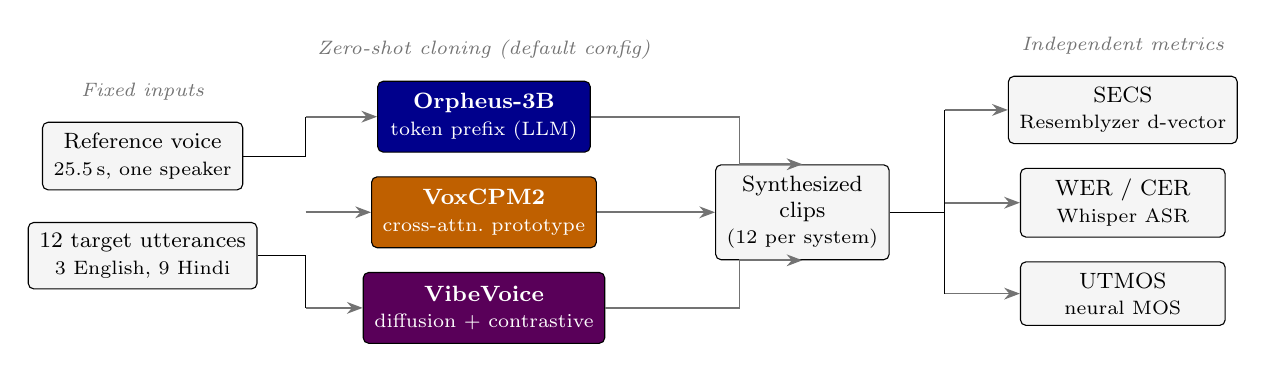
\begin{tikzpicture}[
  font=\footnotesize,
  >={Stealth[length=2mm]},
  box/.style={draw, rounded corners=2pt, align=center, inner sep=4pt, minimum height=8mm},
  io/.style={box, fill=black!4},
  sysbase/.style={box, text=white, minimum width=27mm, minimum height=9mm},
  metric/.style={box, fill=black!4, minimum width=26mm},
  lbl/.style={font=\scriptsize\itshape, text=black!55},
  arr/.style={->, semithick, black!55},
]
\node[io] (ref) {Reference voice\\\scriptsize 25.5\,s, one speaker};
\node[io, below=4mm of ref] (txt) {12 target utterances\\\scriptsize 3 English, 9 Hindi};
\node[lbl, above=1.5mm of ref] {Fixed inputs};
\coordinate (inhub) at ([xshift=7mm]$(ref.east)!0.5!(txt.east)$);

\node[sysbase, fill=blue!55!black, right=17mm of ref, yshift=5mm] (s1)
   {\textbf{Orpheus-3B}\\\scriptsize token prefix (LLM)};
\node[sysbase, fill=orange!75!black, below=3mm of s1] (s2)
   {\textbf{VoxCPM2}\\\scriptsize cross-attn.\ prototype};
\node[sysbase, fill=violet!70!black, below=3mm of s2] (s3)
   {\textbf{VibeVoice}\\\scriptsize diffusion + contrastive};
\node[lbl, above=1.5mm of s1] {Zero-shot cloning (default config)};

\node[io, right=15mm of s2] (out) {Synthesized\\clips\\\scriptsize (12 per system)};

\node[metric, right=15mm of out, yshift=13mm] (m1) {SECS\\\scriptsize Resemblyzer d-vector};
\node[metric, below=3mm of m1] (m2) {WER / CER\\\scriptsize Whisper ASR};
\node[metric, below=3mm of m2] (m3) {UTMOS\\\scriptsize neural MOS};
\node[lbl, above=1.5mm of m1] {Independent metrics};

\draw (ref.east) -- (inhub |- ref.east);
\draw (txt.east) -- (inhub |- txt.east);
\draw (inhub |- ref.east) -- (inhub |- s1.west);
\draw (inhub |- txt.east) -- (inhub |- s3.west);
\draw[arr] (inhub |- s1.west) -- (s1.west);
\draw[arr] (inhub |- s2.west) -- (s2.west);
\draw[arr] (inhub |- s3.west) -- (s3.west);

\draw[arr] (s1.east) -| ([xshift=-8mm]out.north) -- (out.north);
\draw[arr] (s2.east) -- (out.west);
\draw[arr] (s3.east) -| ([xshift=-8mm]out.south) -- (out.south);

\coordinate (outhub) at ([xshift=7mm]out.east);
\draw (out.east) -- (outhub);
\draw (outhub |- m1.west) -- (outhub |- m3.west);
\draw[arr] (outhub |- m1.west) -- (m1.west);
\draw[arr] (outhub |- m2.west) -- (m2.west);
\draw[arr] (outhub |- m3.west) -- (m3.west);
\end{tikzpicture}
\caption{The evaluation protocol. A single reference recording and one fixed
set of target utterances drive all three systems, each run at its released
default configuration with no per-speaker adaptation. Every synthesized clip
is scored by the same three metric models, none of which shares components
with any system under test, so differences in the reported numbers reflect
the synthesis systems. System colours are reused in all later figures.}
\label{fig:pipeline}
\end{figure*}

\subsection{Reference Voice and Target Corpus}
\label{sec:method-corpus}

All three systems clone the same reference recording of one speaker: 25.5
seconds of mono speech, inside the 20--30 second window that zero-shot
systems are typically prompted with. The recording has a mean fundamental
frequency of 118.8~Hz with a standard deviation of 13.9~Hz, a voiced-frame
ratio of 0.66, and an estimated signal-to-noise ratio of 48~dB. Using one
reference for every system removes speaker selection as a confound: any
variation in measured identity preservation reflects what each system does
with the same evidence, not differences in how much evidence it was given.

The target corpus is twelve short, goal-directed utterances of the kind
produced by automated spoken-response systems, three in English and nine in
Hindi. We chose utterances that stress a clone rather than ones that would
maximize fluency scores. Several contain alphanumeric identifiers and spoken
numbers (ticket-style codes, reference numbers, monetary amounts, dates),
because these are the tokens on which an intelligibility metric is most
discriminating: a single dropped or hallucinated digit changes the meaning
while barely perturbing prosody. The Hindi items are written in romanized
Latin script, with transliterated Hindi interleaved with English loanwords,
which is how such prompts are usually authored in practice. That choice has
direct consequences for how Hindi intelligibility has to be scored, discussed
in Section~\ref{sec:method-metrics}. Utterance durations after synthesis span
roughly 4 to 15 seconds. The language split is deliberately asymmetric, nine
Hindi items to three English, because English serves as the
well-characterized control condition and Hindi is the object of study.

\subsection{Systems Under Evaluation}
\label{sec:method-systems}

Each system implements a different approach to speaker conditioning, as set
out in Section~\ref{sec:related-evolution}. We evaluate all three as publicly
released, without architectural modification.

\textbf{Orpheus-3B} is a $\sim$3-billion-parameter language-model-based TTS
system (the \texttt{orpheus-3b-0.1-pretrained} release). It treats speech as
a sequence of discrete audio tokens and conditions cloning on a reference
prefix, so identity is carried entirely by the backbone's in-context learning
and decoded through a neural audio codec.

\textbf{VoxCPM2} is a $\sim$2-billion-parameter codec language model that
replaces the prefix strategy with cross-attention to a fixed speaker
representation extracted from the reference, an intermediate design between
pure prompting and an explicit embedding bottleneck.

\textbf{VibeVoice} is a $\sim$1.5-billion-parameter diffusion-based system
whose decoder is guided by a contrastively trained speaker encoder rather
than an autoregressive codec, placing it in the representation-learning
branch of the literature.

Every system received the same reference clip and target sentences and ran
with its released default inference configuration. No per-speaker adaptation,
per-sentence prompt engineering, or output cherry-picking was applied.

\subsection{Evaluation Metrics}
\label{sec:method-metrics}

Each clip is scored on three complementary axes, plus a set of acoustic
descriptors. Every metric model is independent of all three systems under
test, so no system is scored by a component of its own pipeline.

\textbf{Speaker similarity (SECS).} We embed the reference and each
synthesized clip with the Resemblyzer speaker encoder, a GE2E-style d-vector
network \cite{variani2014deep} trained for speaker discrimination and
unrelated to any of the TTS systems, and report the cosine similarity between
the two 256-dimensional utterance embeddings. Both signals are resampled to
16~kHz mono before embedding. The absolute scale of such cosine scores is
encoder-specific, so the SECS values here are meaningful for ranking the
three systems under one encoder, but should not be compared directly against
speaker-similarity numbers computed with a different encoder such as
ECAPA-TDNN or WavLM.

\textbf{Intelligibility (WER / CER).} Every clip is transcribed with Whisper
(the \texttt{small} model, beam size 5, with voice-activity filtering)
\cite{radford2023whisper} and compared against the input text. Both sides
pass through a normalization stage before scoring: case folding, punctuation
removal, mapping of spelled-out English numbers to digits, and merging of
single-character alphanumeric runs so that a spoken code (``B~4~7~2~9'') and
its written form (``B4729'') are scored as the same content rather than as a
formatting difference. The Hindi measurement chain is necessarily longer, and
we treat it as such. Whisper emits Hindi in Devanagari while our references
are romanized, so we transliterate the hypothesis back to Latin script
(Devanagari~$\rightarrow$~IAST, the deterministic direction) and then apply a
phonetic normalization that collapses romanization-convention noise:
diacritics, vowel-length spellings, \textit{w}/\textit{v} alternation, and
doubled consonants. We report \textbf{WER} as the primary intelligibility
number for English and \textbf{CER} for Hindi. At the word level, schwa
deletion and spelling variation push Hindi WER above 1.0 in many clips,
whereas character-level comparison separates phoneme fidelity from
tokenization artifacts. Because this pipeline depends on a multilingual ASR
model of modest size and a rule-based romanization step, the Hindi error
rates should be read as intelligibility \emph{as measured under this ASR
pipeline}, not as an ASR-independent ground truth.

\textbf{Naturalness (UTMOS).} Naturalness is scored with UTMOS
\cite{saeki2022utmos}, a non-intrusive neural mean-opinion-score predictor
that maps a waveform to a 1--5 scale without a reference signal or a
listening panel. UTMOS was trained predominantly on English and Japanese
listening-test data, so its Hindi scores carry a calibration caveat that we
return to when interpreting the cross-lingual results.

\textbf{Acoustic descriptors.} We also extract simple signal descriptors for
each clip: fundamental-frequency mean and standard deviation via
probabilistic YIN, the absolute pitch deviation from the reference
($|\Delta F_0|$), an SNR estimate, speaking rate, loudness, and
voiced/silence ratios. Of these, $|\Delta F_0|$ is the most diagnostic for
cloning, since a stable clone should reproduce the reference speaker's
register.

\subsection{Aggregation and Scope}
\label{sec:method-scope}

Metrics are computed per clip and then averaged within each system. Because
the central question is cross-lingual, we report English and Hindi means
separately rather than pooling them; word- and character-error rates in
particular are not comparable across the two scripts. This is a controlled,
small-scale comparison: one speaker, one reference, twelve utterances, and a
single generation run per system. We therefore report descriptive results and
effect sizes rather than significance tests, and read the numbers as evidence
about these systems under this protocol rather than as a powered benchmark
claim.

% =================================================================
% Section IV: Results
% =================================================================
\section{Results}
\label{sec:results}

Table~\ref{tab:overall} gives the headline comparison across all four
measured dimensions, and Table~\ref{tab:crosslingual} breaks the identity,
intelligibility, and naturalness axes down by language.
Figure~\ref{fig:overview} plots the three primary axes,
Figure~\ref{fig:tradeoff} the identity--naturalness trade-off by language,
Figure~\ref{fig:dist} the per-clip spread behind the means, and
Figure~\ref{fig:pitch} pitch fidelity. No single system is best on every
axis; the results are better described as a set of trade-offs than as an
overall ranking.

\begin{table}[t]
\caption{Overall system comparison, averaged over all clips except where a
language is specified. Arrows give the improving direction; \textbf{bold} marks
the best value per column. WER is reported for English and CER for Hindi (see
Section~\ref{sec:method-metrics}).}
\label{tab:overall}
\centering
\renewcommand{\arraystretch}{1.2}
\begin{tabular}{lccccc}
\hline
\textbf{System} & \textbf{SECS} & \textbf{UTMOS} & \textbf{WER} & \textbf{CER} & \textbf{$|\Delta F_0|$} \\
 & $\uparrow$ & $\uparrow$ & (En)$\downarrow$ & (Hi)$\downarrow$ & (Hz)$\downarrow$ \\
\hline
Orpheus-3B & 0.894 & 3.51 & 0.116 & 0.548 & 17.7 \\
VoxCPM2 & \textbf{0.948} & 3.73 & \textbf{0.079} & \textbf{0.416} & \textbf{2.5} \\
VibeVoice & 0.933 & \textbf{3.80} & 0.490 & 0.551 & 6.1 \\
\hline
\end{tabular}
\end{table}

\begin{table}[t]
\caption{Cross-lingual breakdown (English, $n=3$; Hindi, $n=9$). Hindi WER is
shown in parentheses but is not the primary Hindi number, as word-level scoring of
romanized Hindi is unreliable (values frequently exceed 1.0).}
\label{tab:crosslingual}
\centering
\renewcommand{\arraystretch}{1.2}
\setlength{\tabcolsep}{4pt}
\begin{tabular}{llcccc}
\hline
\textbf{System} & \textbf{Lang.} & \textbf{SECS}$\uparrow$ & \textbf{UTMOS}$\uparrow$ & \textbf{WER}$\downarrow$ & \textbf{CER}$\downarrow$ \\
\hline
\multirow{2}{*}{Orpheus-3B} & English & 0.897 & 3.83 & 0.116 & 0.074 \\
 & Hindi & 0.893 & 3.41 & (0.983) & 0.548 \\
\hline
\multirow{2}{*}{VoxCPM2} & English & 0.952 & 3.99 & 0.079 & 0.034 \\
 & Hindi & 0.947 & 3.65 & (0.857) & 0.416 \\
\hline
\multirow{2}{*}{VibeVoice} & English & 0.930 & 3.90 & 0.490 & 0.267 \\
 & Hindi & 0.934 & 3.77 & (1.017) & 0.551 \\
\hline
\end{tabular}
\end{table}

\begin{figure*}[t]
\centering
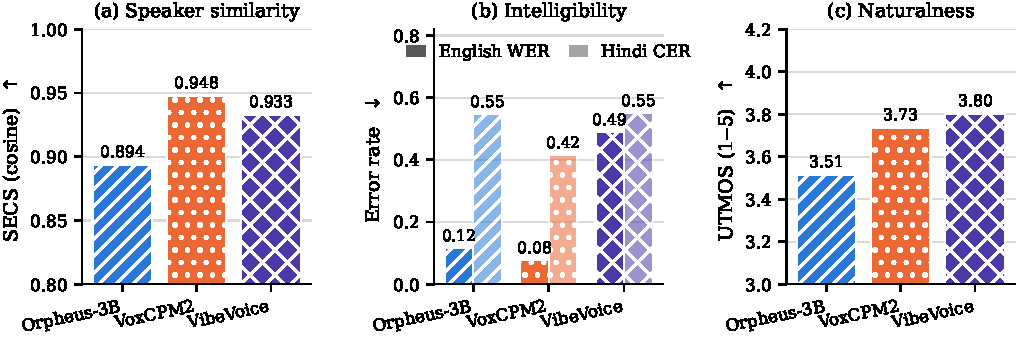
\includegraphics[width=\textwidth]{figures/fig_overview}
\caption{The three primary evaluation axes. (a) Speaker similarity (SECS,
cosine, all clips); (b) intelligibility, contrasting English WER with Hindi
CER; (c) naturalness (UTMOS). Each system keeps the same colour and hatch in
all figures.}
\label{fig:overview}
\end{figure*}

\subsection{Speaker Similarity}
\label{sec:results-secs}

VoxCPM2 preserves speaker identity most faithfully, with a mean SECS of
0.948, followed by VibeVoice at 0.933 and Orpheus-3B at 0.894
(Table~\ref{tab:overall}, Fig.~\ref{fig:overview}a). The gap between the best
and worst system, 0.054 in cosine similarity, is the clearest separation on
any identity-related axis. The per-clip scores tell the same story:
Figure~\ref{fig:dist}a shows VoxCPM2's twelve clips clustered tightly around
its mean, while Orpheus-3B's are both lower and more dispersed, ranging from
about 0.85 to 0.93. Orpheus-3B is thus both the weakest and the least
consistent of the three on identity.

Speaker similarity is almost unaffected by language within each system: the
English and Hindi SECS means differ by at most 0.005 for any system
(Table~\ref{tab:crosslingual}, Fig.~\ref{fig:crosslingual}a). Whatever
mechanism each architecture uses to carry identity from the reference clip
transfers across the two scripts essentially intact, even though, as shown
next, intelligibility does not. Identity preservation and linguistic fidelity
appear largely decoupled in these systems.

\begin{figure}[t]
\centering
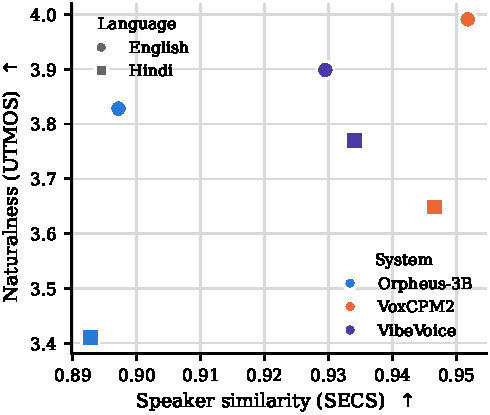
\includegraphics[width=\columnwidth]{figures/fig_tradeoff}
\caption{The identity--naturalness trade-off. Each point is a system's mean
over one language (circles: English; squares: Hindi). VoxCPM2 sits at the
high-similarity edge, VibeVoice at the high-naturalness edge, and Orpheus-3B
is dominated on both.}
\label{fig:tradeoff}
\end{figure}

\subsection{Intelligibility}
\label{sec:results-intel}

On English, where WER is directly interpretable, VoxCPM2 is again strongest
(WER 0.079), Orpheus-3B is close behind (0.116), and VibeVoice is markedly
higher (0.490). The VibeVoice figure is driven by two of its three English
clips: one rendered a numeric ticket code as ``B~fold~729'' and another
drifted on a spoken date, while the third clip matched the best systems at
WER 0.036. With only three English items, we report this as an observation
about specific numeric and alphanumeric utterances rather than as a
distributional claim, though it does match the corpus design intent that
spoken codes are where intelligibility diverges.

The dominant effect in the data is the cross-lingual gap. Hindi character
error rates are far higher than English word error rates for every system
(VoxCPM2 0.416, Orpheus-3B 0.548, VibeVoice 0.551; Fig.~\ref{fig:overview}b),
and character error rates alone rise roughly four- to eight-fold from English
to Hindi (Table~\ref{tab:crosslingual}). Two causes are entangled here, and
we are careful not to attribute the whole gap to synthesis. Part of it is
genuine difficulty: Hindi's retroflex consonants, schwa deletion, and heavy
loanword content are harder to render cleanly, and the per-clip spread in
Figure~\ref{fig:dist}b is correspondingly wide. Part of it is measurement:
the Hindi score passes through a modest multilingual ASR model and a
rule-based Devanagari-to-Latin romanization, and both inject error that
inflates CER independently of audio quality. The ranking among systems is
consistent enough to be informative, with VoxCPM2 leading on Hindi as it does
on English, but the absolute Hindi numbers should be read with the pipeline
of Section~\ref{sec:method-metrics} in mind.

\begin{figure*}[t]
\centering
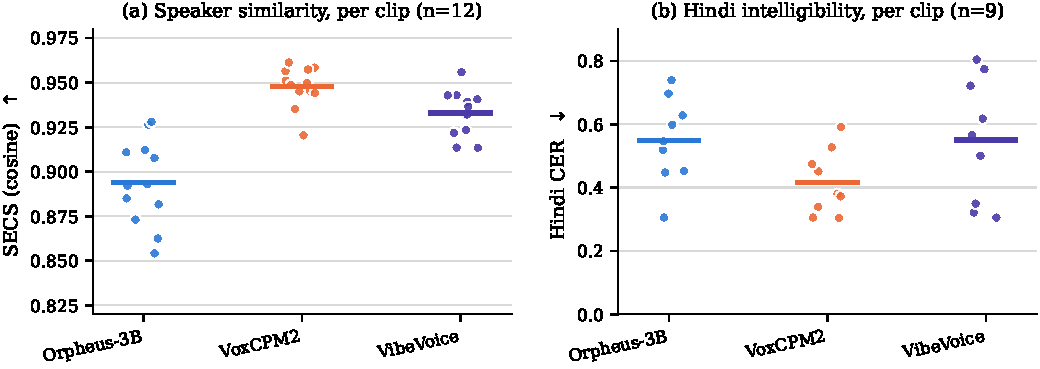
\includegraphics[width=\textwidth]{figures/fig_distributions}
\caption{Per-clip spread behind the means. Horizontal bars mark the
per-system mean. (a) SECS over all 12 clips; VoxCPM2 is both highest and
tightest. (b) Hindi CER over the 9 Hindi clips; VoxCPM2 is lowest, and every
system shows substantial clip-to-clip variation.}
\label{fig:dist}
\end{figure*}

\subsection{Naturalness}
\label{sec:results-utmos}

Predicted naturalness is the axis on which the three systems are most alike.
UTMOS means fall in a narrow band from 3.51 (Orpheus-3B) to 3.80 (VibeVoice),
with VoxCPM2 between them at 3.73 (Fig.~\ref{fig:overview}c). VibeVoice, the
diffusion-based system, scores highest on this predictor and is also the most
stable across languages, losing only 0.13 UTMOS from English to Hindi,
whereas Orpheus-3B and VoxCPM2 drop by about 0.4 and 0.3 respectively
(Table~\ref{tab:crosslingual}, Fig.~\ref{fig:crosslingual}b). Since UTMOS is
not calibrated on Hindi, we read the Hindi values as within-study relative
indicators rather than as absolute mean-opinion scores.
Figure~\ref{fig:crosslingual} places the two axes side by side: the
speaker-similarity lines stay nearly flat across the language boundary while
the naturalness lines slope downward. This is the clearest single view of the
identity/content split that Section~\ref{sec:discussion} builds on.

\begin{figure*}[t]
\centering
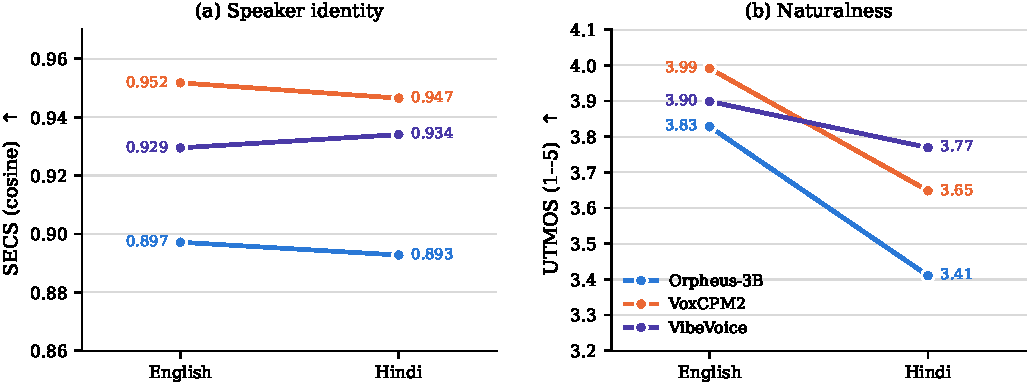
\includegraphics[width=0.72\textwidth]{figures/fig_crosslingual}
\caption{Cross-lingual stability, English versus Hindi, one line per system.
(a) Speaker similarity barely moves across the language boundary (at most
0.005 within any system); (b) naturalness drops for all systems but by
different amounts: 0.13 UTMOS for VibeVoice against about 0.34 and 0.42 for
VoxCPM2 and Orpheus-3B.}
\label{fig:crosslingual}
\end{figure*}

\begin{figure}[t]
\centering
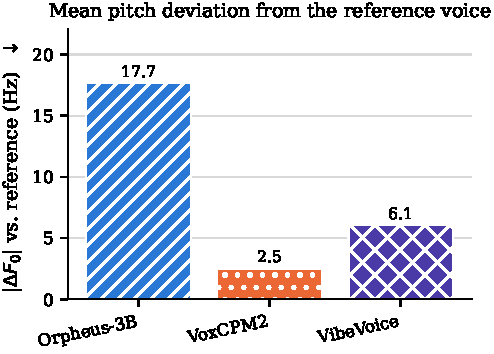
\includegraphics[width=0.85\columnwidth]{figures/fig_pitch}
\caption{Mean absolute deviation of synthesized pitch from the reference
voice's fundamental frequency. VoxCPM2 tracks the reference register almost
exactly, while Orpheus-3B shifts it by nearly 18~Hz.}
\label{fig:pitch}
\end{figure}

\subsection{Pitch Fidelity and the Overall Trade-off}
\label{sec:results-pitch}

The acoustic descriptors support the identity ranking. VoxCPM2 reproduces the
reference speaker's register almost exactly, with a mean
fundamental-frequency deviation of just 2.5~Hz, against 6.1~Hz for VibeVoice
and 17.7~Hz for Orpheus-3B (Fig.~\ref{fig:pitch}). Since $|\Delta F_0|$ is an
absolute quantity, it hides the direction of the error, and the direction is
itself informative. Figure~\ref{fig:pitchreg} plots the raw per-clip pitch
against the reference: Orpheus-3B does not scatter symmetrically around it
but sits above it on every clip, while VoxCPM2 clusters tightly on the
reference line and VibeVoice straddles it more loosely. This register shift
lines up with Orpheus-3B's lower and more variable SECS. The system that
departs most from the reference pitch is also the one that scores lowest on
embedding-based identity.

\begin{figure}[t]
\centering
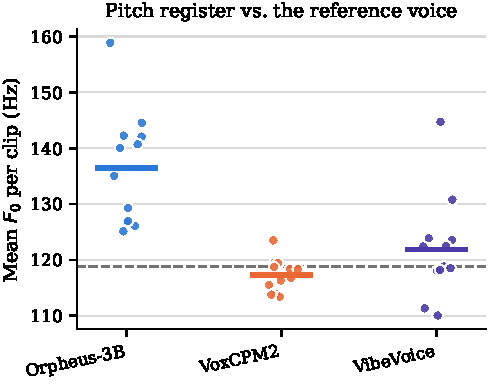
\includegraphics[width=0.85\columnwidth]{figures/fig_pitch_register}
\caption{Per-clip mean fundamental frequency for each system against the
reference voice (dashed line, 119~Hz); horizontal bars mark per-system means.
Unlike the absolute $|\Delta F_0|$ of Fig.~\ref{fig:pitch}, this view shows
direction: Orpheus-3B raises the register on every clip, VoxCPM2 tracks the
reference, and VibeVoice varies around it.}
\label{fig:pitchreg}
\end{figure}

Taken together (Fig.~\ref{fig:tradeoff}), the systems occupy distinct
positions rather than a single ordering. VoxCPM2 is best or tied-best on
speaker similarity, on English and Hindi intelligibility, and on pitch
fidelity, at a small cost in predicted naturalness. VibeVoice is the most
natural and the most language-stable, but has the weakest intelligibility.
Orpheus-3B is dominated on the identity and pitch axes and sits in the middle
on intelligibility and naturalness. Section~\ref{sec:discussion} relates
these positions back to the three conditioning mechanisms described in
Section~\ref{sec:introduction}.

% =================================================================
% Section V: Discussion
% =================================================================
\section{Discussion}
\label{sec:discussion}

The results in Section~\ref{sec:results} separate into two largely
independent stories: how well a system holds onto the speaker, and how
faithfully it renders the words. A system can do well on one and poorly on
the other, and the data show exactly that.

Identity behaves in a way we did not anticipate. Within every system, the
English and Hindi SECS means sit within 0.005 of each other
(Table~\ref{tab:crosslingual}). Whatever each architecture does to carry the
speaker from the reference clip into new speech works about as well in a
language the reference speaker never used, at least for this speaker and this
encoder. Intelligibility shows the opposite pattern: every system loses
heavily moving from English to Hindi, with character error rates rising
roughly four- to eight-fold.

This dissociation constrains how the Hindi error rates should be read. If a
system were genuinely losing its grip on the speaker when it switched to
Hindi, we would expect the identity embedding to move as well, and it does
not. The speaker-conditioning path and the content-generation path fail
independently, which suggests that a substantial part of the Hindi CER gap is
measurement rather than synthesis: the Whisper-small transcription and the
rule-based Devanagari-to-Latin step (Section~\ref{sec:method-metrics}) both
introduce errors that have nothing to do with whether the voice sounds like
the reference. SECS, scored by a pipeline that never touches the ASR chain,
stays flat. We take this as the clearest sign in our data that the two axes
measure different things and fail for different reasons.

The identity axis also has a concrete acoustic correlate, which is reassuring
given how abstract a cosine distance in embedding space is. The
pitch-deviation ranking matches the SECS ranking exactly. VoxCPM2 tracks the
reference register to within 2.5~Hz and takes the top identity score;
Orpheus-3B shifts the register by nearly 18~Hz and takes the bottom one;
VibeVoice sits in the middle on both. The Orpheus-3B shift is not random: it
raises pitch on every clip (Fig.~\ref{fig:pitchreg}), so the drift is a
systematic property of the system rather than clip-level noise, and the
d-vector embedding appears sensitive to it. A listener who perceived
Orpheus-3B as pitched up relative to the reference and the embedding that
scores it lower would be reacting to the same property.

The conditioning mechanisms described in Section~\ref{sec:introduction} offer
a plausible explanation for the identity ranking, though with three systems
we can only note that the results are consistent with it, not prove it.
Orpheus-3B carries the speaker as a token prefix and then generates
autoregressively, so the only route back to the reference is the backbone's
in-context memory, which has to survive a long decoding rollout with no
dedicated pathway to the original evidence. VoxCPM2 keeps a fixed speaker
representation and cross-attends to it at every step, so the reference
remains available late in generation rather than only at the start. That
VoxCPM2 is both highest and tightest on SECS while Orpheus-3B is lowest and
most dispersed (Fig.~\ref{fig:dist}a) is what one would expect if persistent
access to the speaker matters more than the raw capacity of the backbone
holding it in context.

VibeVoice illustrates a different trade-off. Its diffusion decoder produces
the highest UTMOS and the most language-stable naturalness, losing only 0.13
crossing into Hindi against roughly 0.3 to 0.4 for the two codec-based
systems. At the same time it has the weakest intelligibility of the three, in
both languages: an English WER of 0.490 and the highest Hindi CER at 0.551.
The English figure rests on a very small sample, since two of its three
English clips carried numeric or alphanumeric content and both stumbled on it
while the third matched the best systems, so we do not put weight on its
magnitude. The Hindi CER, however, supports the same ranking on separate
data. The overall pattern fits what a diffusion decoder optimizes for: a
smooth, natural waveform rather than the exact discrete tokens that spell out
a code or a date. Rendering a digit correctly is an all-or-nothing target,
and a codec language model with a token-level objective appears to handle it
more reliably than a decoder operating over continuous acoustic trajectories.

None of this yields a single best system, and forcing one would misrepresent
the data. VoxCPM2 is the reasonable default when identity and register
fidelity are the priority: it wins or ties on speaker similarity, on English
and Hindi intelligibility, and on pitch, and it pays only a small and
arguably inaudible price in predicted naturalness. VibeVoice is the better
choice where fluent, natural delivery matters more than verbatim accuracy and
where cross-lingual stability is valued, provided the text is not dense with
codes and numbers. Orpheus-3B, on this protocol, is dominated on identity and
pitch and roughly average elsewhere; its LLM-prefix design is conceptually
the simplest of the three but, in practice, the loosest at holding a voice.

These readings carry the limits the design imposes. The comparison rests on
one speaker, one reference clip, and twelve utterances scored in a single
generation run, so we report effect sizes and describe trade-offs rather than
claim statistical significance (Section~\ref{sec:method-scope}). The English
intelligibility numbers in particular rest on three clips and should be read
as observations about specific numeric utterances. UTMOS is uncalibrated on
Hindi, so the Hindi naturalness scores are within-study indicators, not
absolute opinion scores. And the Hindi error rates include whatever the
ASR-and-romanization chain contributes on top of genuine synthesis error; the
dissociation argument above suggests that contribution is substantial, but it
does not let us subtract it cleanly. What the study does support is narrower
and, we think, still useful: on matched inputs and matched metrics,
persistent cross-attention to a speaker prototype held identity better than
an autoregressive prefix, a diffusion decoder traded token-level accuracy for
naturalness, and speaker identity transferred across scripts far more readily
than linguistic content did.

% =================================================================
% Section VI: Conclusion
% =================================================================
\section{Conclusion}
\label{sec:conclusion}

We compared three zero-shot voice cloning systems, Orpheus-3B, VoxCPM2, and
VibeVoice, under a single controlled protocol: the same reference recording,
the same twelve English and Hindi utterances, and the same
speaker-similarity, intelligibility, and naturalness pipelines for every
system. No system won on every axis. VoxCPM2 held the speaker's identity and
register most tightly and was the most intelligible in both languages.
VibeVoice scored highest on naturalness and changed least across the language
boundary. Orpheus-3B trailed on identity and pitch without leading anywhere
else.

Three findings seem robust despite the study's small scale. Persistent
cross-attention to a fixed speaker prototype preserved identity better than
conditioning on an autoregressive prefix, and the difference had an audible
correlate in how faithfully each system tracked the reference pitch. The
diffusion decoder produced the most natural and most language-stable speech
but was the least reliable at rendering exact content such as digits and
codes. And speaker identity crossed from English into Hindi almost unchanged
while intelligibility did not, a dissociation that separates the two failure
modes and indicates that much of the measured Hindi error belongs to the
ASR-and-romanization scoring chain rather than to the synthesis itself.

Future work follows from the limitations. The single-speaker,
twelve-utterance design should be widened to many speakers and references,
with enough items per language to support significance testing rather than
effect sizes. The naturalness and intelligibility proxies need grounding
against human listeners, especially for Hindi, where UTMOS is uncalibrated
and the CER pipeline does measurable work of its own; a Hindi-native ASR
model and evaluation targets written in Devanagari would help separate
synthesis quality from transcription noise. Broadening the language set
beyond a single Indic language would show whether the ranking of conditioning
mechanisms observed here is a general property or an artifact of this
particular pair. Finally, we would like to probe the mechanisms directly by
swapping prefix conditioning for cross-attention within one architecture,
holding everything else fixed, to test the claim that persistent access to
the speaker, rather than the size of the model holding it, is what keeps a
cloned voice in register.

% =================================================================
% References
% =================================================================
\bibliographystyle{IEEEtran}
\bibliography{references}

\end{document}
